\section{Trip travel times}
\label{sec:trip_state_link}


\begin{knitrout}\small
\definecolor{shadecolor}{rgb}{0.969, 0.969, 0.969}\color{fgcolor}\begin{figure}
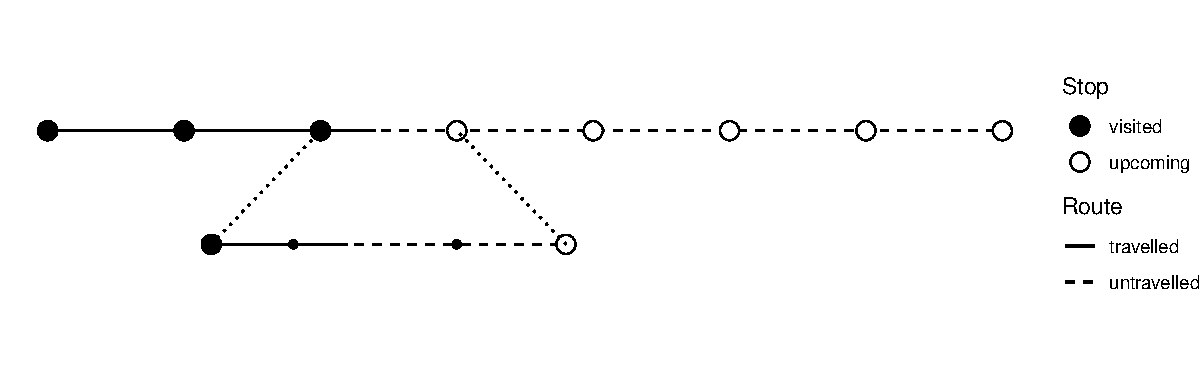
\includegraphics[width=\maxwidth]{figure/trip_segments-1} \caption[A diagram of a route, showing road segment and stop indices]{A diagram of a route, showing road segment and stop indices.}\label{fig:trip_segments}
\end{figure}


\end{knitrout}





Link travel times are the important factor of bus prediction
missing from the current Auckland \gls{rti} system.
Knowing how long the bus will take to travel between stops,
and which stop it is up to,
lets us estimate with more reliability when the bus will arrive,
as the times estimated in \cref{cha:network_model}
account for \rt{} congestion.


Each link $j$ between stops $j$ and $j+1$ in a given route
consist of one or more road segments
$\RouteSegs_j = \collect{r(j),\,r(j)+1,\, \ldots,\, r(j+1) - 1}$,
so the travel time along a link
is the sum of travel times along each of the segments
at time $t_c$,
\begin{equation}
\label{eq:link_tt}
\Linkt_{j} = \sum_{\ell\in\RouteSegs_j} (\NWstate^\Tripr_c)_\ell
\end{equation}
From \cref{sec:nw_realtime} we have that
the segment travel time of segment $\ell$ is
\begin{equation}
\label{eq:seg_tt_dist}
(\NWstate^\Tripr_c)_\ell \sim
\Normal{(\hat{\NWstate^\Tripr}_{c|c})_\ell}%
{(\NWvar^\Tripr_{c|c})_{\ell,\ell}}
\end{equation}

The mean link travel time is easy to compute,
\begin{equation}
\label{eq:link_tt_mean}
\begin{split}
\E{\Linkt_{j}} &=
\E{\sum_{\ell\in\RouteSegs_j} (\NWstate^\Tripr_c)_\ell}
    = \sum_{\ell\in\RouteSegs_j} \E{(\NWstate^\Tripr_c)_\ell}
    = \sum_{\ell\in\RouteSegs_j} (\hat{\NWstate^\Tripr}_c)_\ell
\end{split}
\end{equation}
and similarly the variance, assuming the correlations are known, is
\begin{equation}
\label{eq:link_tt_var}
\begin{split}
\Var{\Linkt_{j}} &=
\Var{\sum_{\ell\in\RouteSegs_j} (\NWstate^\Tripr_c)_\ell} \\
    &= \sum_{k\in\RouteSegs_j} \sum_{\ell\in\RouteSegs_j}
        \Cov{(\NWstate^\Tripr_c)_k}{(\NWstate^\Tripr_c)_\ell} \\
    &= \sum_{k\in\RouteSegs_j} \sum_{\ell\in\RouteSegs_j}
        (\NWvar^\Tripr_c)_{k,\ell}
\end{split}
\end{equation}

However sometimes we need partial segment travel times,
as mentioned above.
The propotions, as calculated using
\cref{eq:trip_percent_dist,eq:trip_percent_time},
can be included in the above
by setting $\SegProg=1$ in all cases other than the current segment
through which the bus is part way.
Now \cref{eq:link_tt} can be rewritten as
\begin{equation}
\label{eq:link_tt_partial}
\Linkt_{j} =
\sum_{\ell\in\RouteSegs_j} \SegProg_\ell (\NWstate^\Tripr_c)_\ell
\end{equation}
which, when substituted into \cref{eq:link_tt_mean}, yields
\begin{equation}
\label{eq:link_tt_mean_partial}
\E{\Linkt_{j}}
    = \sum_{\ell\in\RouteSegs_j} \SegProg_\ell (\hat\NWstate^\Tripr_c)_\ell
\end{equation}
and for the variance, substituting into \cref{eq:link_tt_var} we get
\begin{equation}
\label{eq:link_tt_var}
\Var{\Linkt_{j}}
    = \sum_{k\in\RouteSegs_j} \sum_{\ell\in\RouteSegs_j}
        \SegProg_k\SegProg_\ell (\NWvar^\Tripr_c)_{k,\ell}
\end{equation}


